\section*{Lecture 7}

\subsection*{1.} Consider the matrix
\[ 
A = \begin{pmatrix}
-1 & 1 & -1 & 0\\
1 & 4 & 0 & 1\\
-1 & 0 & 4 & 1\\
0 & 1 & 1 & 9\\
\end{pmatrix}
.\]
Sketch the Gerschgorin disks and specify the location of the eigenvalues of $A$.
\bigbreak
For disk 1 the center is in $-1$ and the sum of the magnitudes of the other entries in the row is $2$ meaning the radius of the disk is 2. Likewise disk 2 will have a center in 4 and a radius of 2, the same is true for disk 3, whilst disk 4 will have a center in $9$ and a radius of two. This is sketched on \textbf{\autoref{fig:l7_1}}.

\begin{figure} [ht]
  \centering
  \caption{Gerschgorin disks of $A$}
  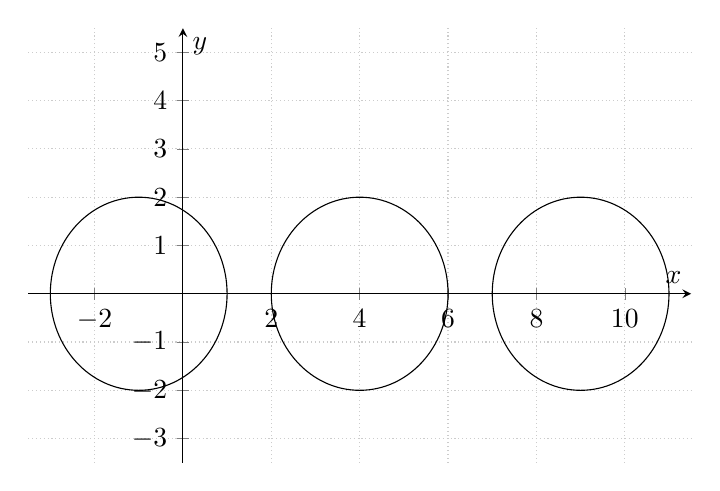
\begin{tikzpicture}
    \begin{axis}[
      width=10cm,
      height=7.1cm,
      axis lines=middle,
      xmin=-3.5,xmax=11.5,ymin=-3.5,ymax=5.5,
      xtick distance=2,
      ytick distance=1,
      xlabel=$x$,
      ylabel=$y$,
      grid=major,
      grid style={thin,densely dotted,black!20}],
    \draw[fill=none](-1,0) circle (2.0);
    \draw[fill=none](4,0) circle (2.0);
    \draw[fill=none](9,0) circle (2.0);
    \end{axis}
  \end{tikzpicture}
  \label{fig:l7_1}
\end{figure}
As $A$ is symmetrical all of its eigenvalues must be real-valued. As the second disk has a ``multiplicity'' of 2 two eigenvalues must be placed here. Therefore 1 eigenvalue is placed in the interval $[-3, 1]$, two eigenvalues are in the interval $[2,6]$ and one eigenvalue is in the interval $[7,11]$. 

\subsection*{2.} Consider the matrix
\[ 
A = \begin{pmatrix}
1 & 0 & 1\\
0 & 1 & 0\\
0 & 0 & 2\\
\end{pmatrix}
.\]
Use the power method with scaling to approximate the largest eigenvalue of $A$ with absolute error less than \num{0,32}.
\bigbreak
For the first approximation I choose 
\[ 
\Vec{x}_0 = \begin{pmatrix}
1\\
1\\
1\\
\end{pmatrix} \implies \Vec{y} = A \Vec{x}_0 = \begin{pmatrix}
2\\
1\\
2\\
\end{pmatrix}
.\]
For the first approximation we get
\begin{align*}
  m_0 &= \Vec{x}^{T} \Vec{x} = \begin{pmatrix}
  1 & 1 & 1\\
  \end{pmatrix} \begin{pmatrix}
  1\\
  1\\
  1\\
  \end{pmatrix} = 3\\
  m_1 &= \Vec{x}^{T} \Vec{y} = \begin{pmatrix}
  1 & 1 & 1\\
  \end{pmatrix} \begin{pmatrix}
  2\\
  1\\
  2\\
  \end{pmatrix} = 5 \\
  m_2 &= \Vec{y}^{T} \Vec{y} = \begin{pmatrix}
  2 & 1 & 2\\
  \end{pmatrix} \begin{pmatrix}
  2\\
  1\\
  2\\
  \end{pmatrix} = 9 
.\end{align*}
We now find the Rayleigh coefficient
\[ 
q = \frac{m_1}{m_0} = \frac{5}{3}
.\]
We therefore get the error
\[ 
\epsilon = |q - \lambda| \leq \delta = \sqrt{\frac{m_2}{m_0} - q^2} = \sqrt{3 - \frac{25}{9}} = \num{0,47} 
.\]
We therefore must try again. We start by scaling as
\[ 
\Vec{x}_1 = \frac{A \Vec{x}_0}{\text{Largest component of } A \Vec{x}_0} = \begin{pmatrix}
1\\
\frac{1}{2}\\
1\\
\end{pmatrix}
.\]
This gives us
\[ 
\Vec{y} = A \Vec{x}_1 = \begin{pmatrix}
2\\
\frac{1}{2}\\
2-\\
\end{pmatrix}
.\]
Now we have the approximation
\begin{align*}
  m_0 &= \Vec{x}^{T} \Vec{x} = \begin{pmatrix}
  1 & \frac{1}{2} & 1\\
  \end{pmatrix} \begin{pmatrix}
  1\\
  \frac{1}{2}\\
  1\\
  \end{pmatrix} = \frac{9}{4} \\
  m_1 &= \Vec{x}^{T} \Vec{y} \begin{pmatrix}
  1 & \frac{1}{2} & 1\\
  \end{pmatrix} \begin{pmatrix}
  2\\
  \frac{1}{2}\\
  2\\
  \end{pmatrix} = \frac{17}{4} \\
    m_2 &= \Vec{y}^{T} \Vec{y} = \begin{pmatrix}
    2 & \frac{1}{2} & 2\\
    \end{pmatrix} \begin{pmatrix}
    2\\
    \frac{1}{2}\\
    2\\
    \end{pmatrix} = \frac{33}{4}
.\end{align*}
We now get the Rayleigh coefficient
\[ 
q = \frac{m_1}{m_0} = \frac{17}{9}
.\]
Which gives the error
\[ 
\epsilon = \left| q - \lambda \right| \leq \delta = \sqrt{\frac{m_2}{m_0} - q^2} = \sqrt{\frac{33}{9} - \frac{289}{81}} \approx \num{0,31} 
.\]
Therefore the largest eigenvalue of $A$ is in the interval $\frac{17}{9} \pm \num{0,31} $


\subsection*{3.} Solve the ODE
\[ 
x^3 + y(x)^3 y'(x) = 0
\]
using the theory of seperable ODEs.
\bigbreak
A seperable ODE can be written on the form
\[ 
y'(x) = \frac{h(x)}{g(y(x))}
.\]
These can be solved with the formula
\[ 
  \int_{y \left( x_0 \right)}^{y(x)} g(y) \, \mathrm{d}y = \int_{x_0}^{x} h \left( \tilde{x} \right) \, \mathrm{d} \tilde{x}
.\]
We can rewrite our ODE as
\[ 
y'(x) = \frac{-x^3}{y(x)^3}
.\]
With $h(x) = -x^3$ and $g(y(x)) = y(x)^3$. We now get
\begin{gather*}
  \int_{y(x_0)}^{y(x)} g(y) \, \mathrm{d}y = \int_{x_0}^{x} h(\tilde{x}) \, \mathrm{d}\tilde{x} \\
  \implies \int_{y(x_0)}^{y(x)} y^3 \, \mathrm{d}y = \int_{x_0}^{x} -\tilde{x}^3 \, \mathrm{d} \tilde{x} \\
  \implies \left[ \frac{y^{4}}{4} \right]_{y(x_0)}^{y(x)} = \left[ - \frac{\tilde{x}^{4}}{4} \right]_{x_0}^{x} \\
  \implies \frac{1}{4} \left( y(x)^{4} - y(x_0)^{4} \right) = \frac{1}{4} \left( x_0^{4} - x^{4} \right) \\
  \implies y(x) = \pm \sqrt[4]{\left( x_0^{4} - x^{4} \right) + y(x_0)^{4}}
.\end{gather*}


\subsection*{4.} Solve the ODE
\[ 
4x + y(x) y'(x) = 0
\]
using the theory of seperable ODEs. Find the solution that fulfills $y(2) = 3$.
\bigbreak
We rewrite as
\[ 
y'(x) = \frac{-4x}{y(x)}
.\]
We can now once again use the formula
\[ 
  \int_{y(x_0)}^{y(x)} g(y) \, \mathrm{d}y = \int_{x_0}^{x} h(\tilde{x}) \, \mathrm{d}\tilde{x}
.\]
However we must remember to set $x_0 = 2, y(x_0) = y(2) = 3$. Doing this we get
\begin{gather*}
\int_{3}^{y(x)} y \, \mathrm{d}y = \int_{2}^{x} -4 \tilde{x} \, \mathrm{d}\tilde{x} \\
\implies \left[ \frac{y^2}{2} \right]_3^{y(x)} = \left[ -2 \tilde{x}^2 \right]_2^{x} \\
\implies \frac{1}{2} \left( y(x)^2 - 9 \right) = 8 - 2x^2 \\
\implies y(x) = \pm \sqrt{25 - 4x^2}
.\end{gather*}
However, as $y(2) = 3$, the above just becomes $y(x) = \sqrt{25 - 4x^2}$


\subsection*{5.}
Consider the free fall of a melting snowball described by the ODE (2). Find the solution $v(t)$ corresponding to the initial value $v(0) = 0$, using the theory of seperable ODEs.
